\iffalse
\bibliography{myreference.bib}
\fi

%chapter 5
\chapter{Experimental Results}
In chapter 3, we have prepared the dataset. First we use it to train a linear model using logistic regression.

\section{Feature Selection in CFS}
In the feature vector, there are correlated features. Thus, we need to remove such dependency first. The feature we use in our project are listed in the following table.
\begin{table}[!hbp] \centering \label{Tab:featurevector}
\begin{tabular}{|c|c|c|c|}
\hline
Emotion & HasURL & Length & RealWord \\
\hline
ImgWord & EngWord & OtherWord & RegPostTime \\
\hline
Verified & VerifiedType & VerifiedKind & Gender \\
\hline
GeoEnabled & Province & FollowersCount & FriendsCount \\
\hline
BiFollowersCount & StatusesCount & FavouritesCount & CommentCount \\
\hline
ShareCount & AttributesCount &  &  \\
\hline
\end{tabular}
\caption{Feature Vector}
\end{table}
After selection, only 7 features are left.
\begin{table}[!hbp] \centering \label{Tab:featurevector}
\begin{tabular}{|c|c|c|c|}
\hline
Emotion & ImgWord & EngWord & VerifiedKind \\
\hline
FollowersCount & BiFollowersCount & ShareCount &\\
\hline
\end{tabular}
\caption{Feature Vector Left}
\end{table}
In the left feature, all of them are continuous feature except the ``VerifiedKind'', which is a nominal feature. To make the logistic regression algorithm can run, we need to transform this nominal feature into several binary features.

In ``VerifiedKind'' feature, there are four category, which is ``normal user'', ``master'', ``yellowV'' and ``blueV''. Thus, we create four new features and drop the original ``VerifiedKind'' feature. So the feature vector becomes
\begin{table}[!hbp] \centering \label{Tab:featurevectorforlr}
\begin{tabular}{|c|c|c|c|}
\hline
Emotion & ImgWord & EngWord & master\\
\hline
yellowV & blueV & normal user & \\
\hline
FollowersCount & BiFollowersCount & ShareCount & \\
\hline
\end{tabular}
\caption{Feature Vector for Training}
\end{table}

\section{Training by Logistic Regression}

We taking this ten features into logistic regression and do standardization. We choose l2-norm regularization and set $C=1.5$. After training, the model is given as the following table with intercept or $\theta_0=-0.36647169$.
\begin{table}[!hbp] \centering \label{Tab:featurevectorforlr}
\begin{tabular}{|c|c|c|c|}
\hline
\textbf{Feature} & \textbf{Coefficient} & \textbf{Feature} & \textbf{Coefficient} \\
\hline
Emotion & -0.38976887 & ImgWord & -0.39248365 \\
\hline
EngWord & -0.45859069 & master & 0.21188558 \\ 
\hline
yellowV & -0.03449316 & blueV & -0.30445247 \\
\hline
normal user & 0.16429209 & FollowersCount & -2.44114483\\
\hline
BiFollowersCount & 0.36734794 & ShareCount & 1.92550177\\
\hline
\end{tabular}
\caption{Coefficient of each feature}
\end{table}

When we train this model, we use $70\%$ of data as the training set and use $30\%$ left to evaluate the performance in Table. \ref{Table:PerformanceofLR}. The overall accuracy is 0.781.
\clearpage
%table of evaluation of logistic regression
\begin{table}[th] \centering 
\begin{tabular}{ccccc}
\toprule
& \textbf{precision} & \textbf{recall} & \textbf{f1-score} & \textbf{support}\\
\midrule
False & 0.81 & 0.75 & 0.78 & 744\\
True  & 0.76 & 0.81 & 0.78 & 704\\
avg/total & 0.78 & 0.78 & 0.78 & 1445\\
\bottomrule
\end{tabular}
\caption{Model Performance trained by Logistic Regression}
\label{Table:PerformanceofLR}
\end{table}

% The confusion matrix is in Table. \ref{Tab:ConfMatoflr}:

% \begin{table}[t] \centering \label{Tab:ConfMatoflr}
% \begin{tabular}{c|cc|c}
% \hline
% & \textbf{True} & \textbf{False} & \textbf{sum} \\
% \hline
% Positive & 570 & 134 & 704 \\
% Negative & 183 & 558 & 741 \\
% \hline
% sum & 692 & 753 & 1445\\
% \hline
% \end{tabular}
% \caption{Confusion matrix of LR model}
% \end{table}

We can take the absolute value of them and draw a histgram in Fig. \ref{fig:ImptbyLR}
%figure of importance by logistic regression
\begin{figure}[h]\centering
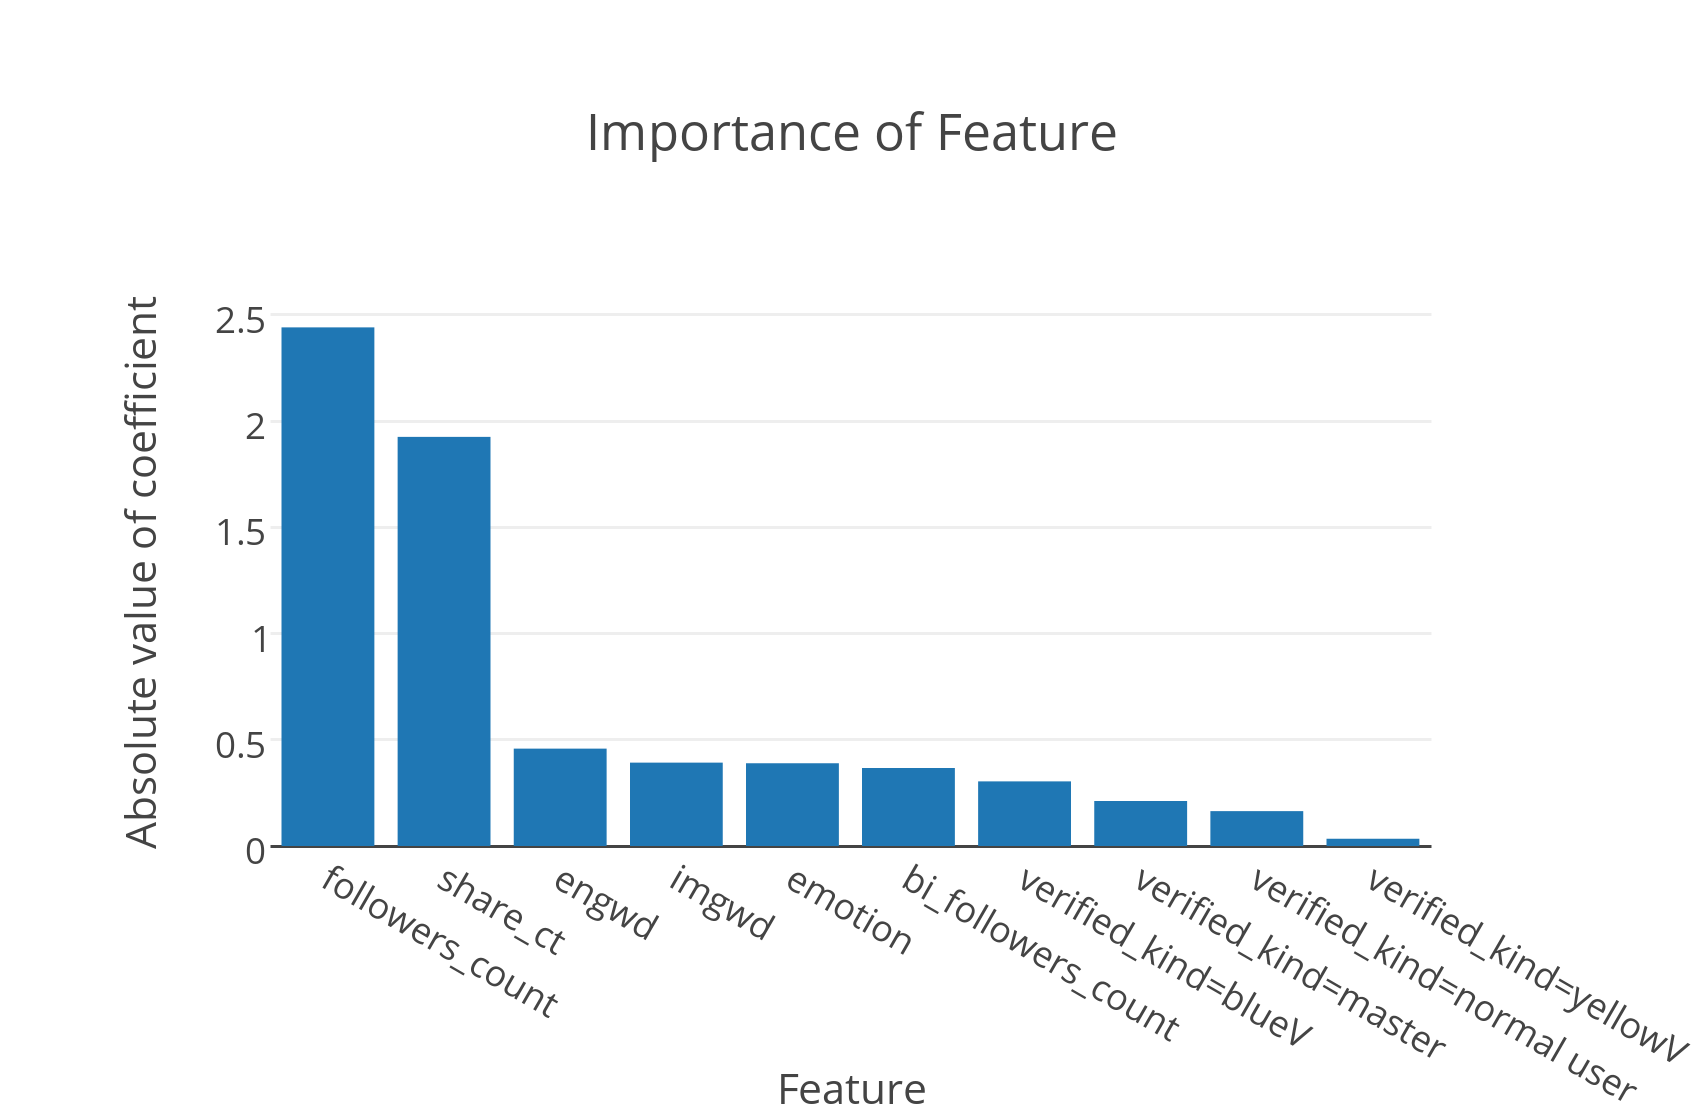
\includegraphics[width=1\textwidth]{imptbyLR}
\caption{Importance of Feature by Logistic Regression} \label{fig:ImptbyLR} \end{figure}

\section{Training by Random Forest}
To support the result from the logistic regression, we train a model using random forest with the same input features. In the algorithm, the number of tree is set as 500. Table \ref{Table:PerformanceofRF} is the evaluation of the trained model using ``30\%'' testset. The accuracy is 0.817. The importance of each feature is drawn in histgram in Fig. \ref{fig:ImptbyRF}
\clearpage
% table of evaluation of random forest based on Gini
\begin{table}[th] \centering 
\begin{tabular}{ccccc}
\toprule
& \textbf{precision} & \textbf{recall} & \textbf{f1-score} & \textbf{support}\\
\midrule
False & 0.82 & 0.82 & 0.82 & 726\\
True  & 0.82 & 0.82 & 0.82 & 719\\
avg/total & 0.82 & 0.82 & 0.82 & 1445\\
\bottomrule
\end{tabular}
\caption{Model Performance trained by Random Forest}
\label{Table:PerformanceofRF}
\end{table}
%figure of importance by Random Forest based on Gini
\begin{figure}[th]\centering
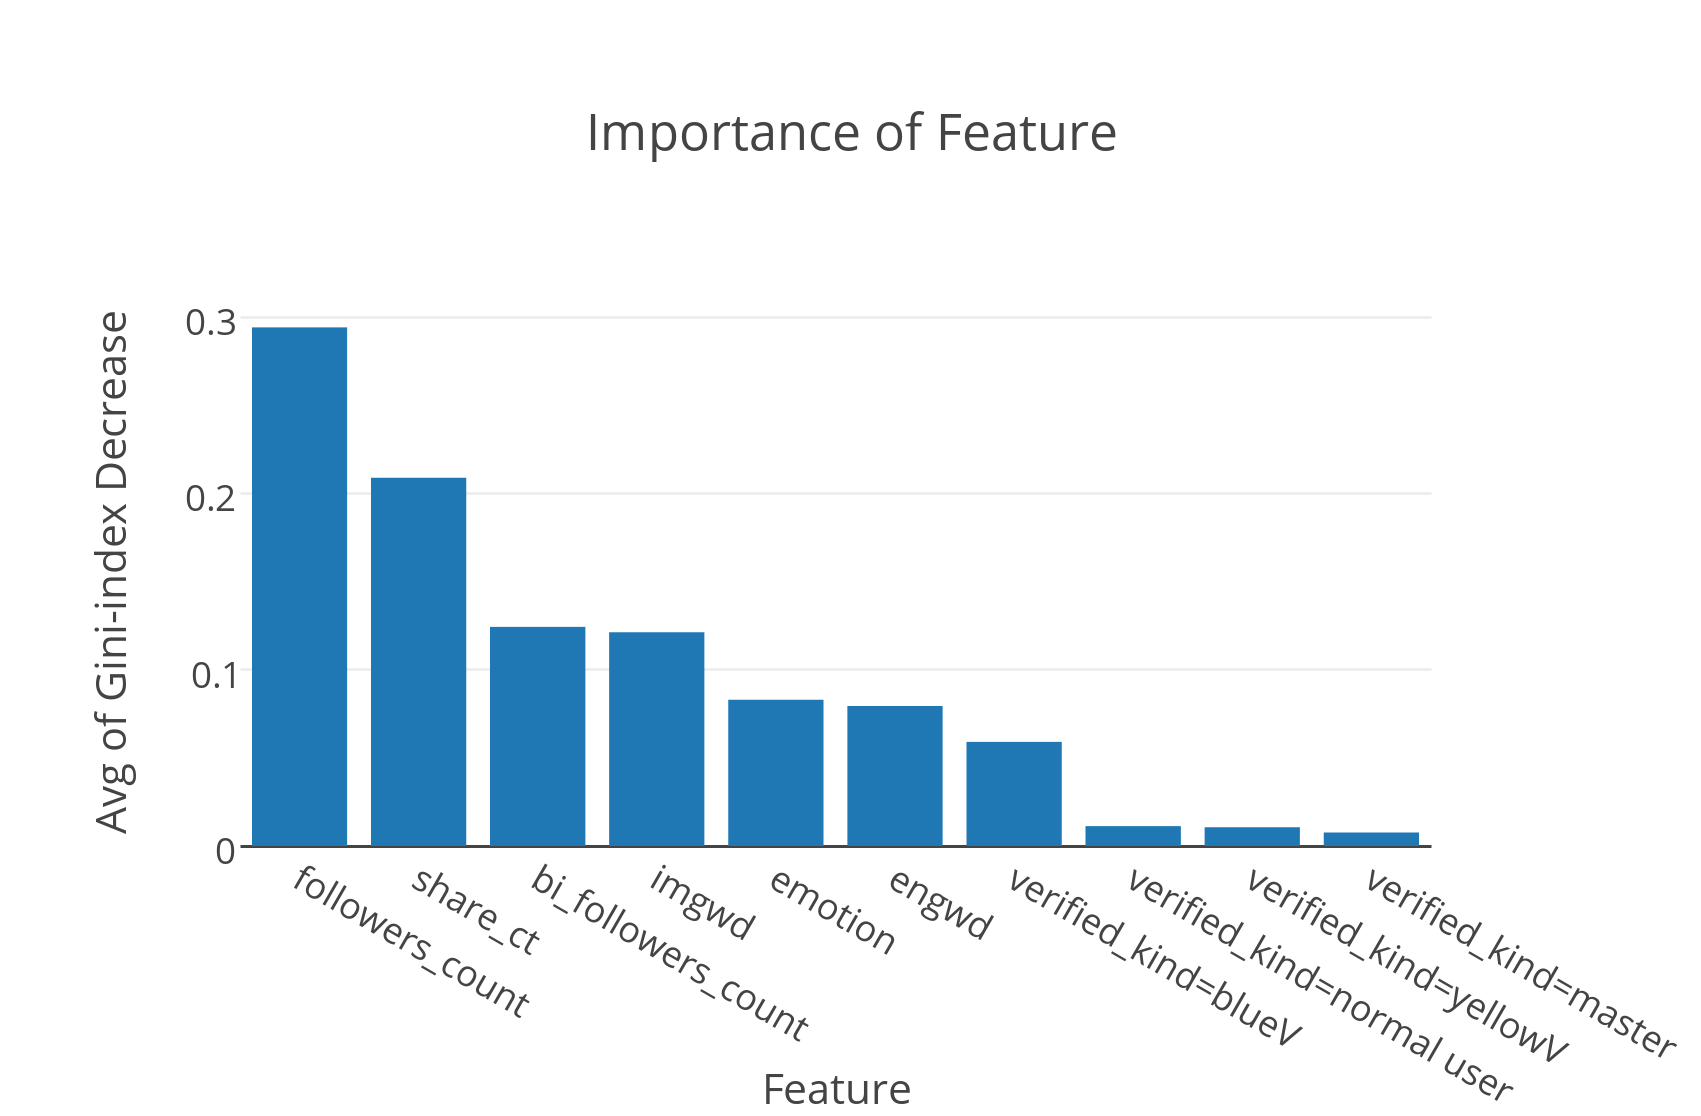
\includegraphics[width=1\textwidth]{imptbyRF}
\caption{Importance of Feature by Random Forest} \label{fig:ImptbyRF} \end{figure}

In Fig. \ref{fig:ImptbyLR} and \ref{fig:ImptbyRF}, ``FollowersCount'' and ``ShareCount'' takes the first and second place, means these two features are most important among these input feature.



% \begin{table}[t] \centering \label{Tab:ConfMatofrf}
% \begin{tabular}{c|cc|c}
% \hline
% & \textbf{True} & \textbf{False} & \textbf{sum} \\
% \hline
% Positive & 587 & 132 & 719 \\
% Negative & 133 & 593 & 726 \\
% \hline
% sum & 692 & 753 & 1445\\
% \hline
% \end{tabular}
% \caption{Confusion matrix of LR model}
% \end{table}





Random forest can reduce the impact from the correlated input feature while the logistic regression cannot. Thus we design a comparison between these two algorithm using all the features we introduce before the CFS procedure and draw two histgrams in Fig. \ref{fig:allFeatbyLR} and Fig. \ref{fig:allFeatbyRF}.
\clearpage
\begin{figure}[t]\centering
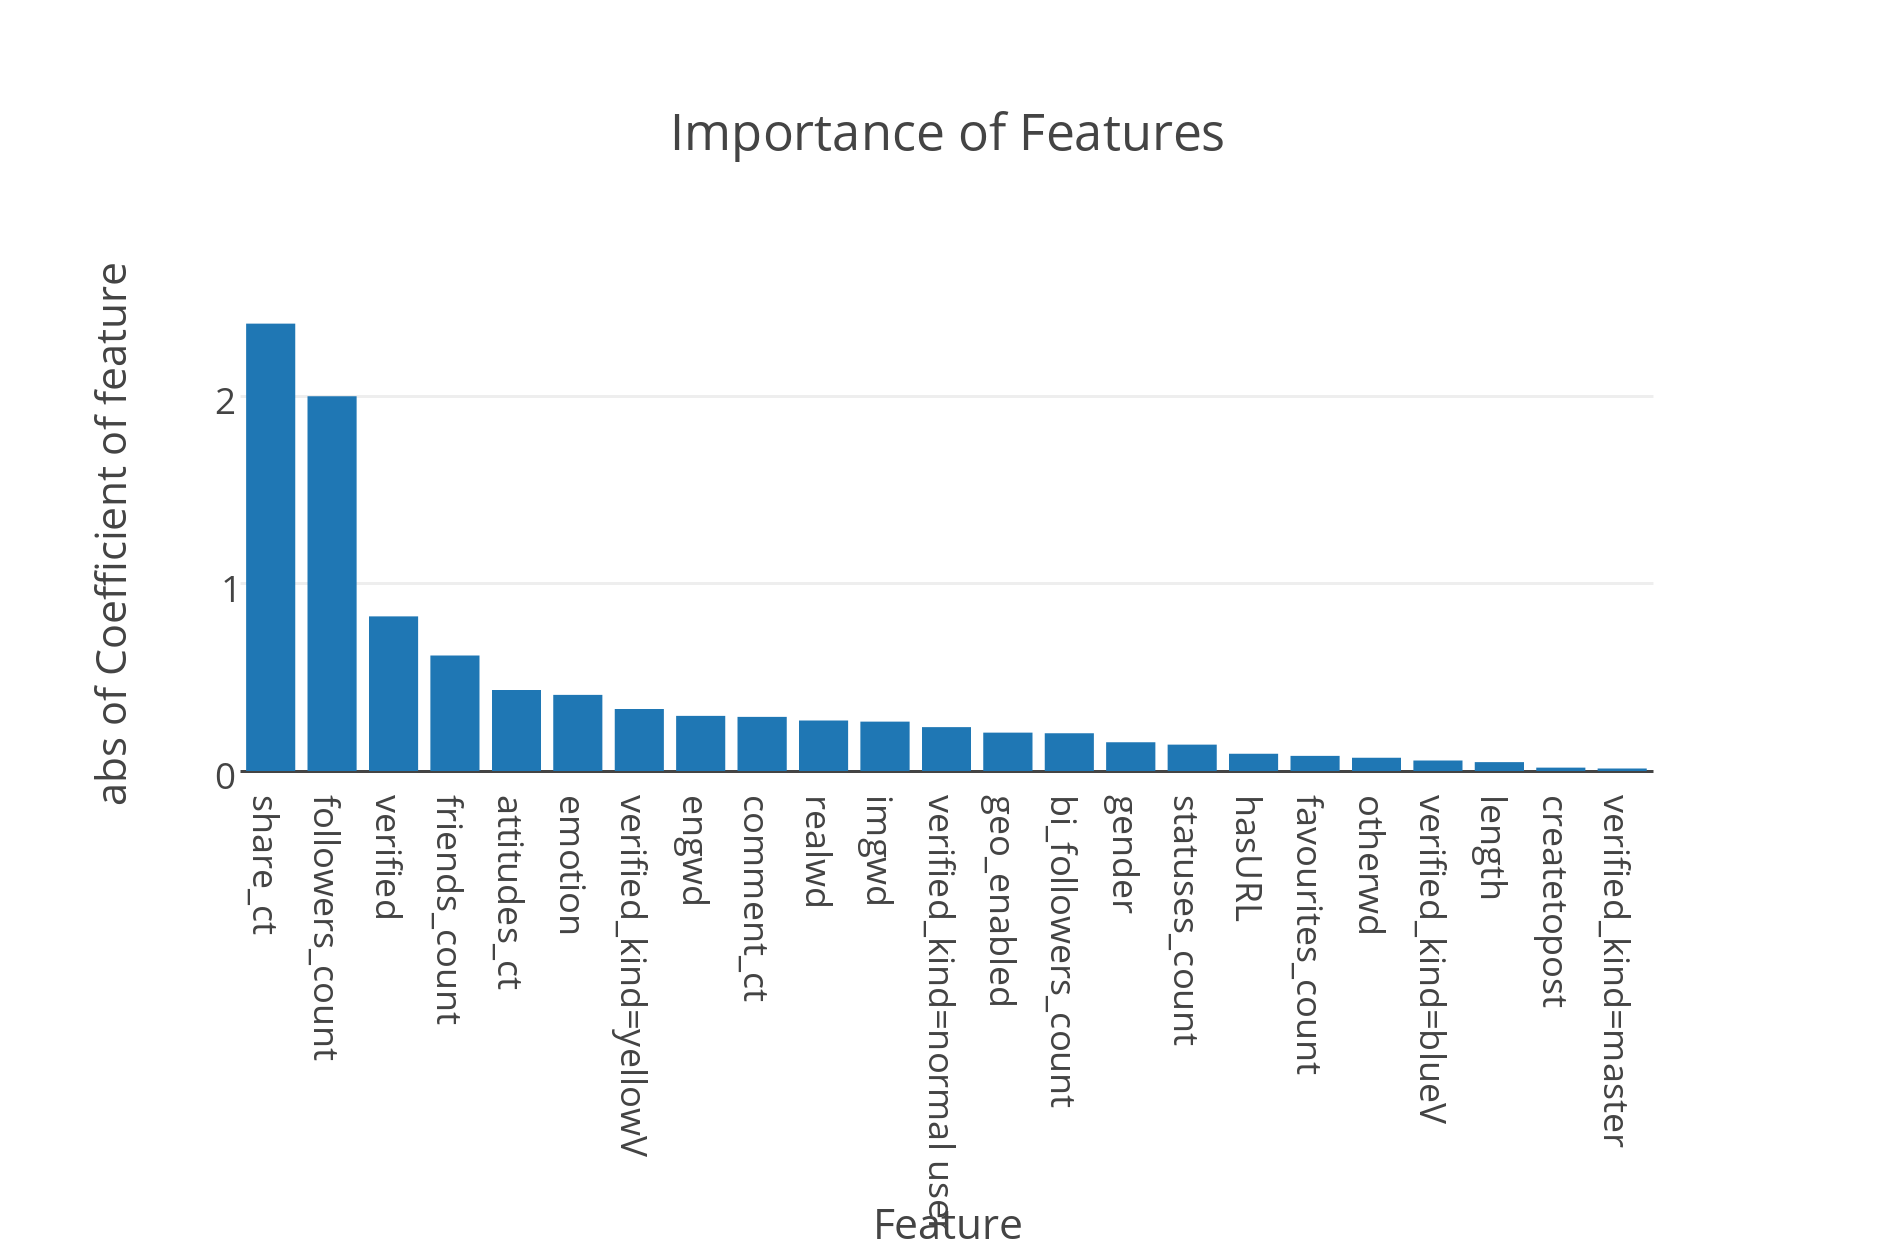
\includegraphics[width=1\textwidth]{allfeatLR}
\caption{All Feature trained by Logistic Regresson} \label{fig:allFeatbyLR} \end{figure}

\begin{figure}[h]\centering
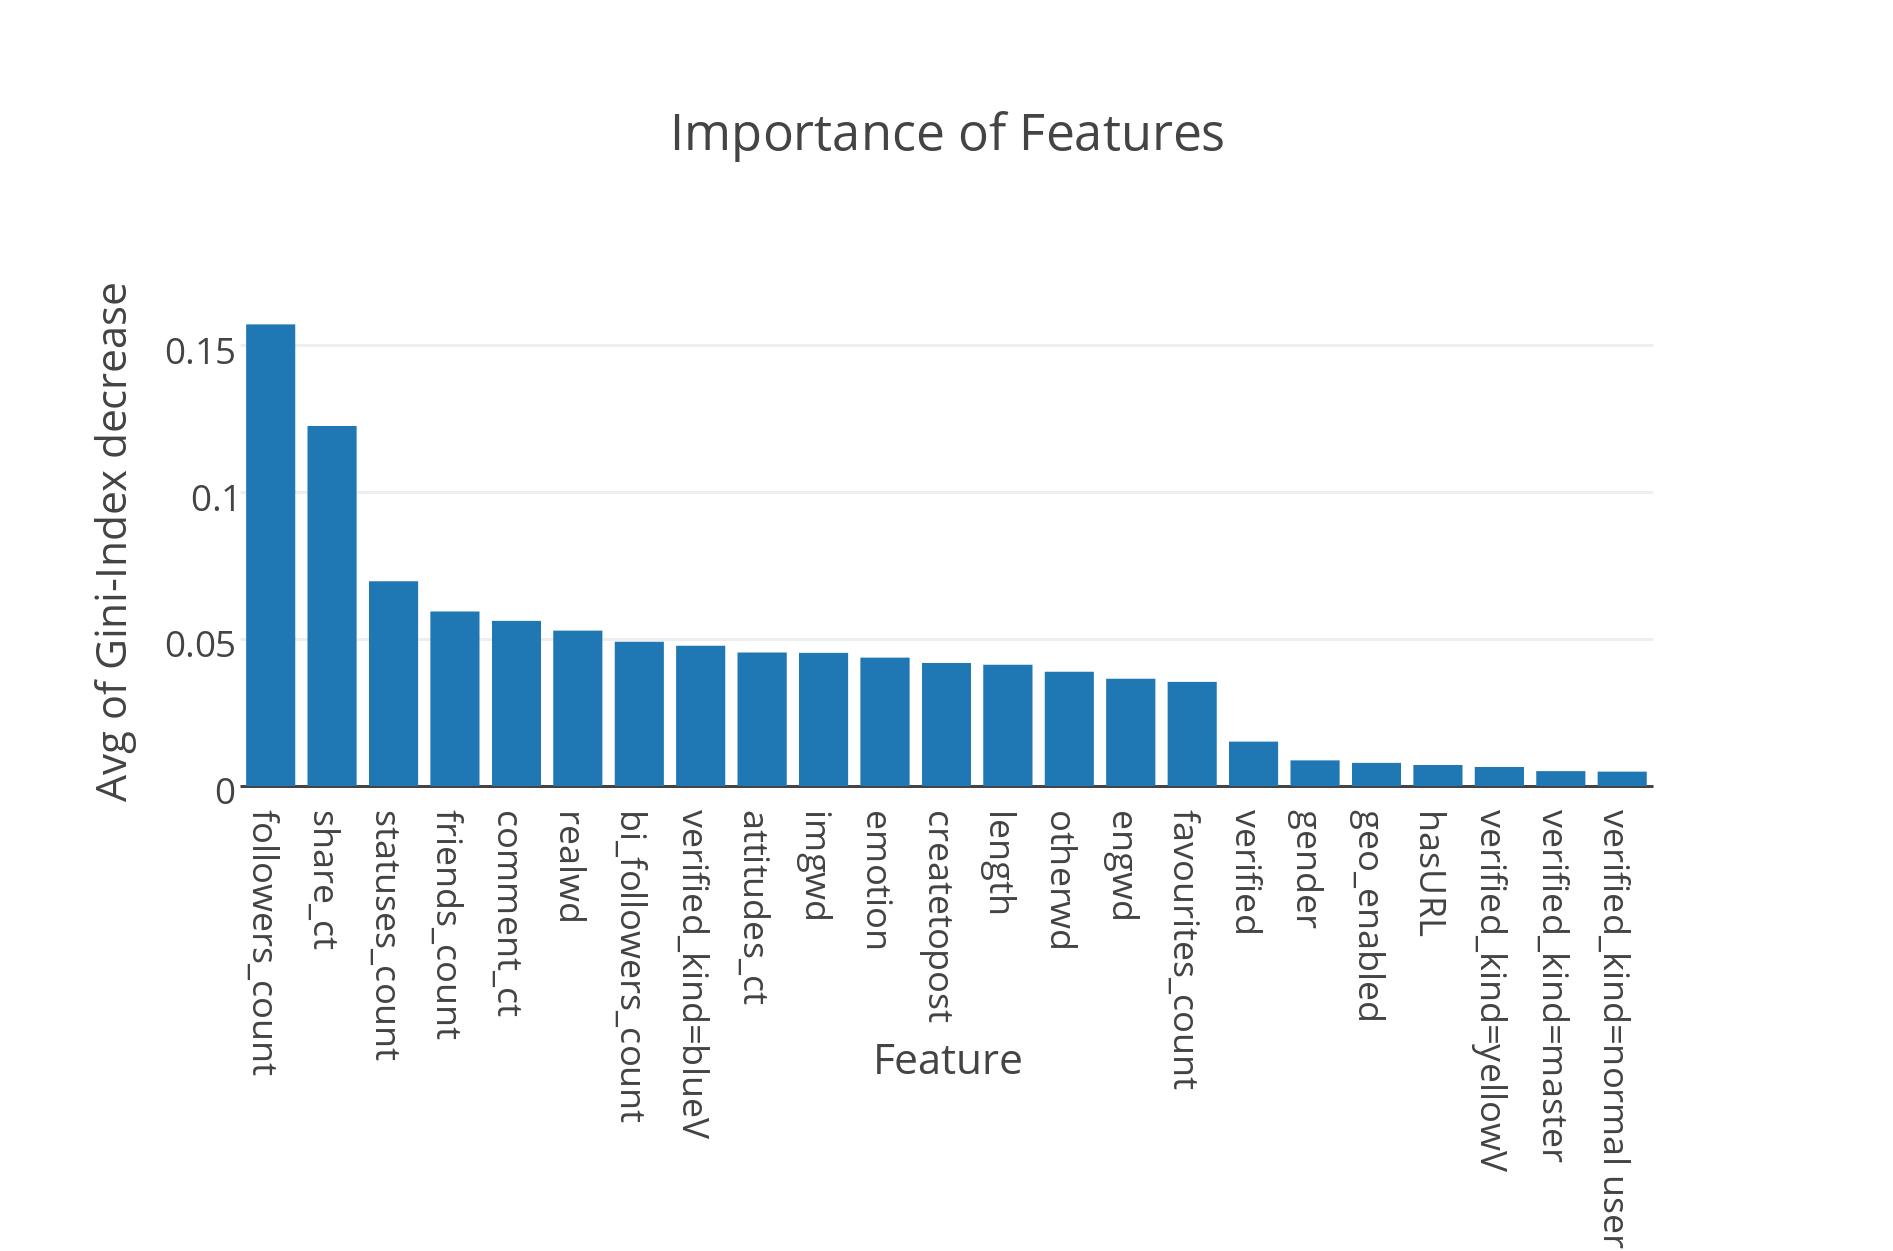
\includegraphics[width=1\textwidth]{allfeatRF}
\caption{All Feature trained by Gini-based Random Forest} \label{fig:allFeatbyRF} \end{figure}

\clearpage
From this two figures, most of the features are disordered each other. Take ``verified'' as the example, which is not be selected by the CFS. It means that this feature is dependent on some other features. Actually it is quite related with the ``VerifiedType'' and ``VerifiedKind'' feature. If taking this feature into the logistic regression training procedure, the coefficient of it may be inaccurate. In Fig. \ref{fig:allFeatbyLR}, the coefficient of ``verified'' is measured as a large value, but actually random forest tells us it should be ranked not at very high pisition in Fig. \ref{fig:allFeatbyRF}.

Even if random forest can reduce the bias from the feature-feature inner-correlation, it has the drawback when dealing with the data including categorical features with different level. It is biased of preferring those features with more categories. For example, we have a nominal type and a numeric type feature. The numeric can be seen as an infinite categories feature compared with the nominal feature. To remove this bias, we run a random forest algorithm to measure the importance of features based on the mean decrease of accuracy when permuting on the data.
\begin{figure}[h]\centering
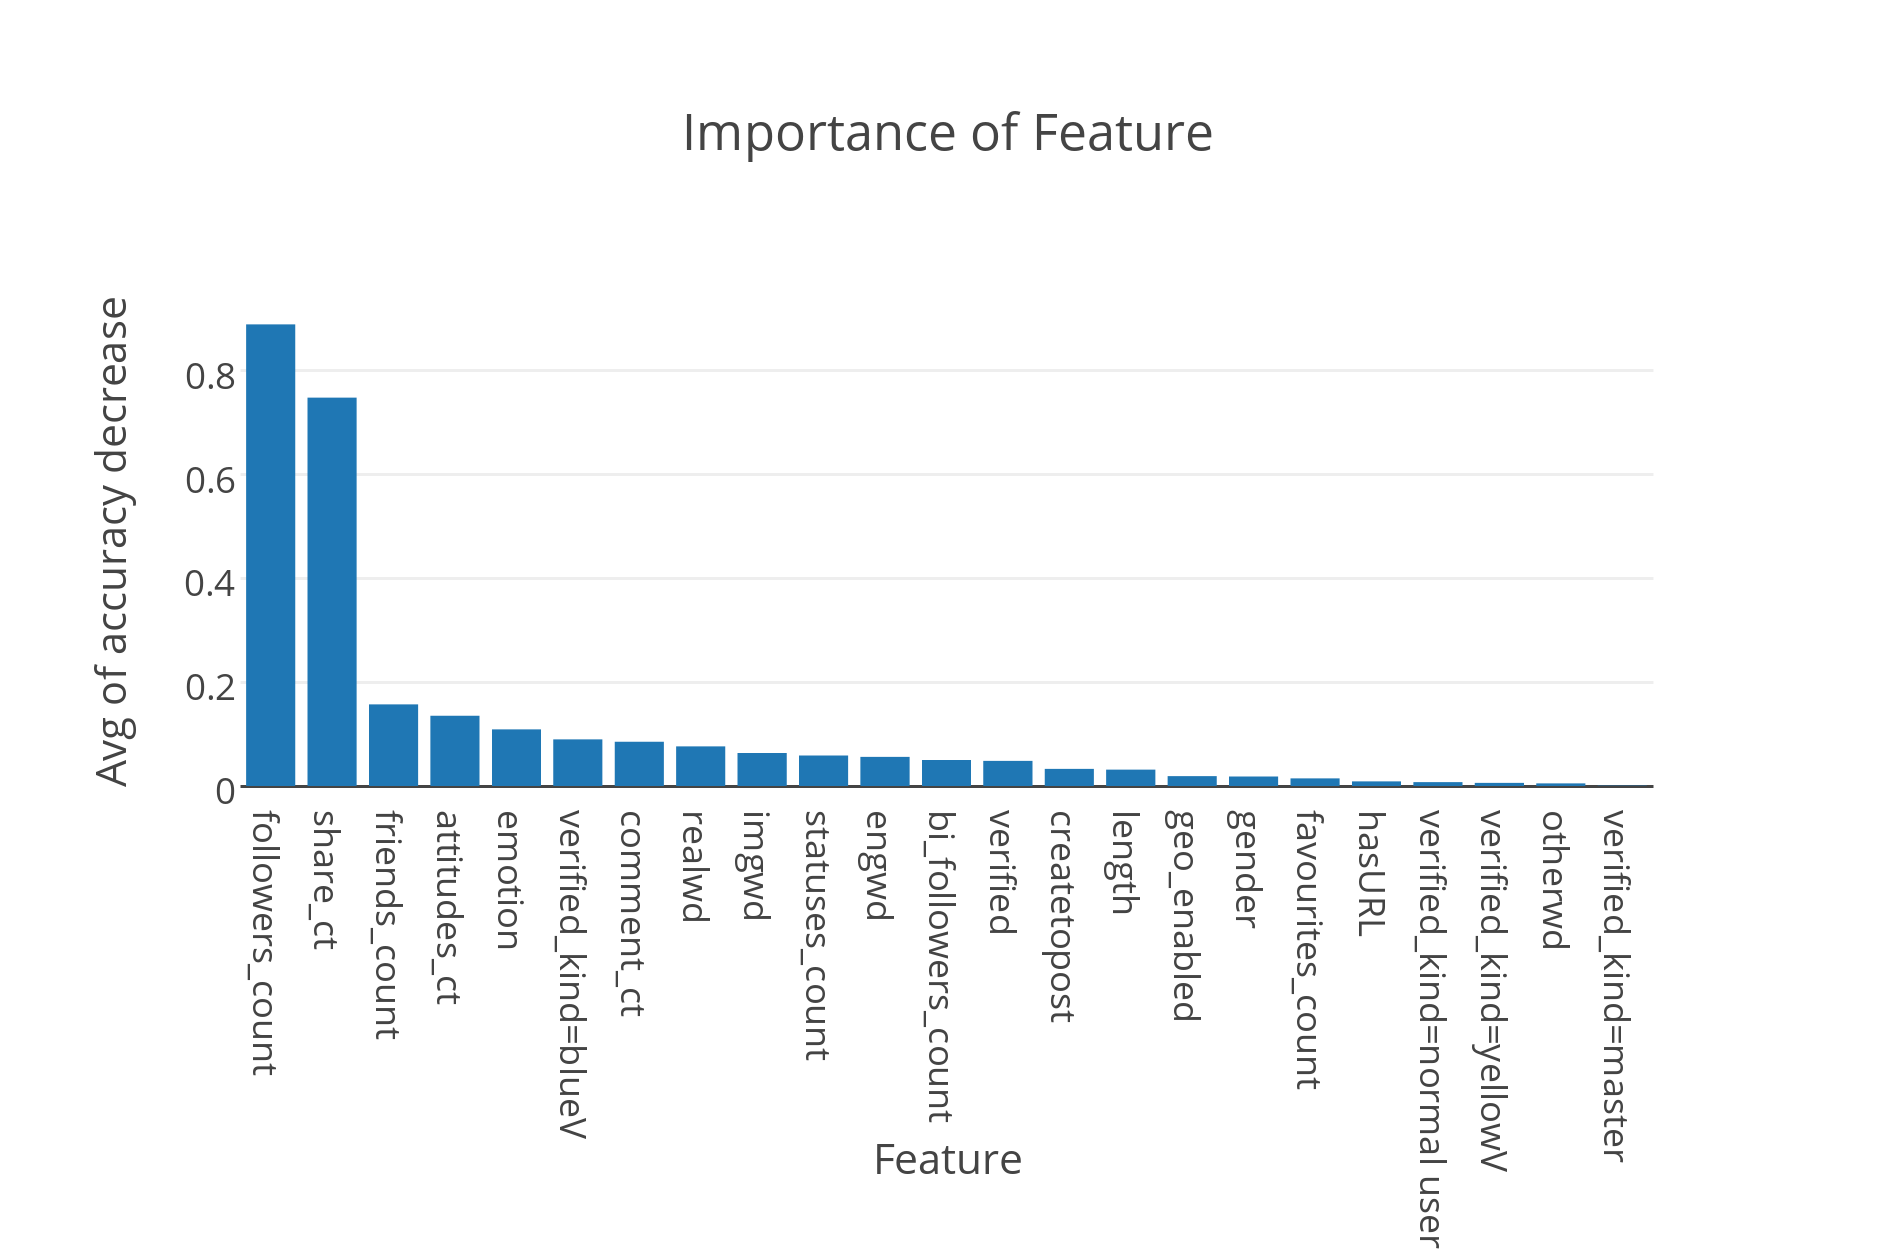
\includegraphics[width=1\textwidth]{AllfeatRFpermutation}
\caption{All Feature trained by Permutation-based Random Forest} \label{fig:ImptbyRFpermutation} \end{figure}

The result is drawn in Fig. \ref{fig:ImptbyRFpermutation}


This figure also indicates the ``FollowersCount'' and ``ShareCount'' have strong incluence on the model performance. Permutating these two features decreases model accuracy by over 80\% and 78\%. We can also see the rank of ``BlueV'' feature increase. Actually if we find the dataset with ``BlueV'', we find that the ratio of rumor and not rumor is $1:5$ among 1132 ``BlueV'' samples. It explains that the ``BlueV'' feature is relatively importance but its score is limited by the small number of sample. 

This method also can work on the situation of correlated input feature because the score of importance is evaluated after the model is trained. We permute only one feature at a time and calculate the score. If the data of correlated feature are permuted one by one, the scores of them are still very close.
